\section{Rubin Observatory Commissioning}
\label{sec:commissioning}

The baseline schedule for on-sky observations with LSSTCam during commissioning includes 3 months of technical integration and testing followed by an 8-week period of sustained observing in the form of one or more Science Validation Surveys \citep{SCTN-007}.

\subsection{Commissioning observations}

\begin{figure}
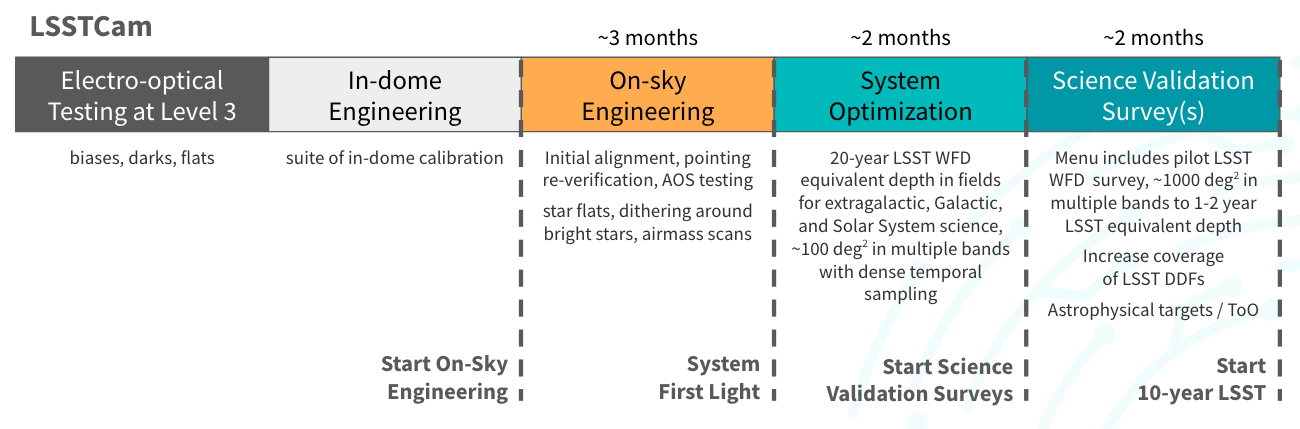
\includegraphics[width=\linewidth]{figures/commissioning-plan}
\caption{Outline plan for the collection of commissioning data, as of October 2022.}
\label{fig:commissioning}
\end{figure}

Figure~\ref{fig:commissioning} shows the high level plan for the Rubin commissioning observations, first with the $40\times40$~arcmin field of view Commissioning Camera ``ComCam,'' and then with the LSST Camera.
Commissioning data collection is planned to take place in phases.
A period of on-sky engineering time will be followed by a set of observations designed to help optimize the system, before the \svs are carried out.
The SV surveys are designed to support scientific analyses that validate the system's performance, and allow Rubin to demonstrate operations readiness.

The figure indicates a number of key components of the system optimization and SV phases planned for each camera.
These include a LSST wide-fast-deep (WFD) 1-2 year equivalent depth ``pilot'' survey.
Field selection will be carried out by the Commissioning Team, taking into account a wide variety of constraints as well as a ``menu'' of science opportunities to which the LSST Science Community has contributed.
Details of the Commissioning plans will be made available as those plans converge, in this technote and other documents as cited.


\subsection{Template generation during commissioning}

By the end of the commissioning period, coadd templates for use in difference imaging will only be available for $\approx$ 10\% of the sky.
Generating templates over a wide area is not an explicit goal of commissioning;  however, where possible, if commissioning observations are agnostic to pointing and filter, we would endeavour to choose a pointing and filter that maximizes building templates to enable early science.
During LSSTCam commissioning we intend to incrementally generate templates over the maximal sky area supported by the available observations.

The LSST SRD places well-defined criteria on the quality of the difference image and the amount of noise that a template can contribute to a difference image.
These criteria result in a minimum of three images being needed to construct a template for use in year one.
The commissioning period provides an excellent opportunity to investigate how many visits in a given band are sufficient to construct a usable template.
Given the desire to maximize the science harvest prior to the \drone,  relaxing these criteria is an option to be explored.


\subsection{Alert generation during commissioning}

Due to the need to verify the instrument characteristics, template quality, and image differencing and Real/Bogus performance, real-time alerts will not be immediately available during the commissioning period.
However, the incremental template generation and alert production processes will be tested and optimized during ComCam and LSST Cam on-sky commissioning, resulting in a set of prompt data products, including alerts.

The ComCam alerts will be {\it canned}, and released to the community as part of DP1 (Table~\ref{tab:dp-one-products}).
Broker teams will be given access to these alerts prior to the DP1 release, but only for development purposes.
The goal for these ComCam canned alerts is to enable alert brokers and science users to understand their characteristics and to help to validate their quality, rather than to enable rapid followup and \es per se.

Templates, alerts, and other prompt data products will also be produced during LSST Cam on-sky commissioning, with the Alert and Prompt Product databases filled and made available for query prior to the DP2 data release (analgous to LSST survey operation, Table~\ref{tab:dp-two-products}). 
Rubin will aim to provide a ``near-live'' alert stream to the Brokers by the end of the LSST Cam SV surveys.


\subsection{Data Previews based on commissioning data}

Data acquired during commissioning that is of science-quality will be released to the Rubin data rights community via two Data Previews, Data Preview 1 (DP1) for data from the commissioning camera (ComCam) and Data Preview 2 (DP2) for data from the LSST science camera (LSSTCam) and all previous commissioning data.
Data Previews will be produced using the DRP pipeline and will include data products for both static sky science and time domain science.
